\begin{center}


\begin{figure}[t]
\centerline{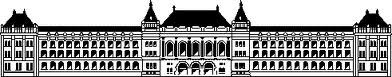
\includegraphics[ width=0.6\textwidth]{bmelogo.png}}
\end{figure}
\textbf{\small{Budapesti Műszaki és Gazdaságtudományi Egyetem\\Matematika Intézet}\\}
\vspace{2cm}

\textbf{\Large {SZAKDOLGOZAT\\}}
\vspace{1 cm}
 \textbf{\Large{Diszkrét maximum-elv végeselem-módszerre\\elliptikus parciális differenciálegyenleteken\\}}
  \vspace{1cm}														
  \textbf{\Large{Balla Réka}\\}
\vspace{3cm}

\begin{tabular}{rcl}  
\textbf{\large{Konzulens:}} & \hspace{1 cm} & \textbf{\large{Karátson János}}\\
  &   & \large{egyetemi tanár,}\\
  &   & \normalsize{ELTE TTK, Alkalmazott Analízis}\\
  &   & \normalsize{és Számításmatematika Tanszék,}\\  
  &   & \normalsize{BME, Analízis Tanszék}
\end{tabular}
 

 
 \vspace{2 cm}
\textbf{\Large{2017}}

\end{center}